\documentclass[conference]{IEEEtran}
\IEEEoverridecommandlockouts
\usepackage[ngerman]{babel}
% The preceding line is only needed to identify funding in the first footnote. If that is unneeded, please comment it out.
\usepackage{cite}
\usepackage{amsmath,amssymb,amsfonts}
\usepackage{algorithmic}
\usepackage{graphicx}
\usepackage{textcomp}
\usepackage{xcolor}
\usepackage{setspace}
\usepackage{booktabs}
\usepackage[export]{adjustbox}
\def\BibTeX{{\rm B\kern-.05em{\sc i\kern-.025em b}\kern-.08em
    T\kern-.1667em\lower.7ex\hbox{E}\kern-.125emX}}
\begin{document}

\title{Currency Exchange, eine App zur Anzeige von Wechselkursen mit Hilfe eines Webscrapers}


\author{\IEEEauthorblockN{1\textsuperscript{st} Matz, Annika}
\IEEEauthorblockA{\textit{dept. name of organization (of Aff.)} \\
\textit{name of organization (of Aff.)}\\
Berlin, Deutschland \\
s\_matz22@stud.hwr-berlin.de}
\and
\IEEEauthorblockN{2\textsuperscript{nd} Liebenberg, Benjamin}
\IEEEauthorblockA{\textit{dept. name of organization (of Aff.)} \\
\textit{name of organization (of Aff.)}\\
Oranienburg, Deutschland \\
s\_liebenberg22@stud.hwr-berlin.de}
\and
\IEEEauthorblockN{3\textsuperscript{rd} Reetz, Tobias}
\IEEEauthorblockA{\textit{dept. name of organization (of Aff.)} \\
\textit{name of organization (of Aff.)}\\
Berlin, Deutschland \\
s\_reetz22@stud.hwr-berlin.de}
%Beispiel wie es aussah
%\and
%\IEEEauthorblockN{3\textsuperscript{rd} Given Name Surname}
%\IEEEauthorblockA{\textit{dept. name of organization (of Aff.)} \\
%	\textit{name of organization (of Aff.)}\\
%	City, Country \\
%	email address or ORCID}
}

\maketitle


\section{Einführung}
Innerhalb unseres dualen Studiums der Informatik an der "Hochschule für Wirtschaft und Recht", nahmen wir an dem Modul Software-Engineering 2 teil. Ziel dieses ist die Entwicklung von Software, vermittelt zu bekommen und das erlernte Wissen direkt anwenden zu können innerhalb einer Projektarbeit. Dabei wird auf die Grundlagen des Projektmanagments geachtet, wofür z.B. UML-Diagrammen angefertigt werden. Zur Dokumentation des Projektes wird dieses Paper angefertigt. 
Innerhalb des Moduls werden auch Softskills gefördert, z.B. die Präsentationsfähigkeiten oder die Sozialkompetenz innerhalb von Gruppenarbeiten.

\section{Idee des Projektes}
Ein sehr großer Teil unseres Lebens dreht sich um das erwerben von unterschiedlichen Materiellen Gütern. Für unserer Arbeit werden wir vergütet, im Supermarkt kaufen wir davon unser Abendessen und an den Wochenenden und im Urlaub gehen wir auf Reisen. Auf diesen müssen wir uns in einer fremden Kultur zu Recht finden und konsumieren weiter Güter. Doch wie können wir einen Wert von diesen einschätzen, wenn wir die Währung nicht kennen? Und genau dieses Problem löst unsere App "Currency Exchange". Einfaches nachschlagen von tagesaktuellen Wechselkursen und umrechnen zwischen verschiedenen Währungen. Ein besonderes Feature ist das Umwandeln des eingegebenen Wertes in die Anzahl von Döner, welche damit gekauft werden könnten in Euro. \\
Die  Android-App arbeitet mit Hilfe eines Webscrapers , welcher Wechselkurse erhält und Beträge der unterschiedlichen Währungen ineinander umrechnet.

\section{Projektorganisation}
Innerhalb eines Softwareentwicklungsprojekts erhalten die einzelnen Bearbeitenden verschiedene Rollen, die ihnen unterschiedliche Aufgaben zu teilen. In diesem Fall bestand das Entwicklungsteam aus wenigen Personen, so wurden keine expliziten Arbeitsbereiche vergeben.  So wurden Aufgaben nach und nach vergeben, wobei jeder Bereich eine eigene Ansprechperson besaß. Unterteilt wurde in Projektleitung, Serveradministration, Design und Testdurchführung. Zu Anfang wurde für essentiell wichtige Themen, wie z.B. die Software-Architektur oder den groben Design-Entwurf, wurden Teammeetings durchgeführt und die Umsetzung so zusammen geplant. Sichergestellt wurde so, dass jedes Teammitglied mit einbezogen wird und alle auf dem gleichen Stand sind. \\
Die Programmierung der Software wurde von Teammeeting zu Teammeeting aufgeteilt. Hauptsächlich kümmerten sich Benjamin und Tobias Reetz um die Programmierung des Webscrapers, sowie die Schnittstelle und ein Teil des Backend der App. Annika Matz kümmert sich vor allem um die Umsetzung des Designentwurfs zu einem funktionierenden Frontend, sowie ein Teil der Programmierung des Backend.

\subsection{Projektleitung}
Der Projektleitung wurde von Annika Matz übernommen. Unteranderem behielt sie die unterschiedlichen Abgabetermine im Blick. Außerdem sorgte sie für regelmäßig Treffen in der Gruppe und leitete diese an. Bei diesen wurde der aktuelle Stand ausgewertet, weitere Entwicklungsschritte besprochen und Aufgaben verteilt. \\
Des weiteren achtete sie auch auf die Projektanforderungen und führte die Qualitätssicherung durch, wodurch sie für eine angemessene Feedback innerhalb der Teammeetings sorgt.

\subsection{Serveradministration}
Der Bereich Serveradministration wurde von Benjamin Liebenberg beaufsichtigt. Aufgrund seiner weitreichenden Erfahrung in diesem Gebiet, konnte er diesen Bereich übernehmen. Er hostet unseren Webscraper auf seinem Server, sorgt für täglich aktualisierte Daten innerhalb der App und stellt die Schnittstelle für unsere App bereit.

\subsection{Design \& Testplanung}
Das Design und die Testplanung wurden zum größten Teil von Tobias Reetz übernommen. Aufgrund seiner Designerfahrung im Modul Software-Engineering 1, übernahm er diese Rolle und designte vor allem das App-Logo. Er sorgte für eine angemessene Farbgebung und dafür, dass die App aufgrund ihrer Gestaltung schnell wieder erkennt werden kann. \\
Außerdem übernahm er das Konkretisieren von Usability-Tests, welche wir zuvor im Plemnum entworfen hatte und führte diese mit unseren Kommilitonen durch. Damit trug er einen entscheidenen Beitrag zur Fehlersuche und somit zur Qualität unseres Programmes bei.

\section{Anforderungen}
An eine Software werden immer unterschiedliche Erwartungen und Anforderungen gestellt. Eine genaue Definition sind wichtig für den Erfolg des Projektes. In diesem Projekt werden die unterschiedlichen Anforderung in drei Kategorien unterteilt. Sie beinhalten nicht funktionale, funktionale und optionale funktionale Anforderungen.

\subsection{Nicht funktionale Anforderungen}
Nicht-funktionale Tests decken alle Anforderungen ab, welche das gesamte System ansich betreffen. Es werden somit keine Funktionen abgeprüft, sondern Eigenschaften und Bestandteile. Für das Projekt wurde besonders auf eine sehr gute Usability geachtet, was besonders durch eine intuitive und einfache Benutzung begründet werden soll.
Desweiteren soll eine Verfügbarkeit des Projekt auf Android-Handys garantiert werden. Um einen hohen Datenschutz garantieren zu können erheben wir keine Daten und speichern auch nicht die in der Vergangenheit getätigten Eingaben dem Nutzer zur Verfügung. 

\subsection{Funktionale Anforderungen}
Funktionale Anforderung definieren die Funktionen und Erwartungen der Software, welche für ein erfolgreiches Projekt erfüllt werden müssen. \\
Das wichtigste Ziel für die Software ist eine lauffähige Android-Handy-Applikation, welche verschiedene Eingaben zwischen verschiedenen Währungen richtig Umrechnen kann. Es soll immer ein tagesaktueller Wechselkurs bereit stehen. In die App sollen auch mindestens sieben Währungen eingebunden werden.

\subsection{Optionale funktionale Anforderungen}
Anforderungen, welche nicht essentiell notwendig für die grundlegenden Funktionsweise sind, aber sie diese erweitern, werden zu den optionalen funktionalen Anforderungen gezählt. \\
Zu diesen zählt die Umrechnung der Anzahl an Döner, die die Nutzenden sich mit dem eingetragenen Wert kaufen könnten in Euro. Außerdem könnte die App durch eine Funktion zum Hinzufügen von Prozentualen Werten ergänzt werden. Diese könnten zum Beispiel zur Berechnung der Mehrwertsteuer oder des Trinkgeldes genutzt werden.

\section{Entwurf}
Innerhalb eines Entwurfs wird der Aufbau und die Struktur des Projektes geplant und fest gehalten. Dieser besteht in diesem Projekt aus zwei der Systemarchitektur, einem Sequenzdiagramm und dem groben Designentwurf. Nach diesen Vorgaben wurde die App entwickelt.

\subsection{Systemarchitektur}
Eine Systemarchitektur beschreibt die Struktur des Projektes, so wie alle seine vorkommenden Bereiche und wie diese miteinander interagieren. 

\begin{figure}[h]
	\centering
	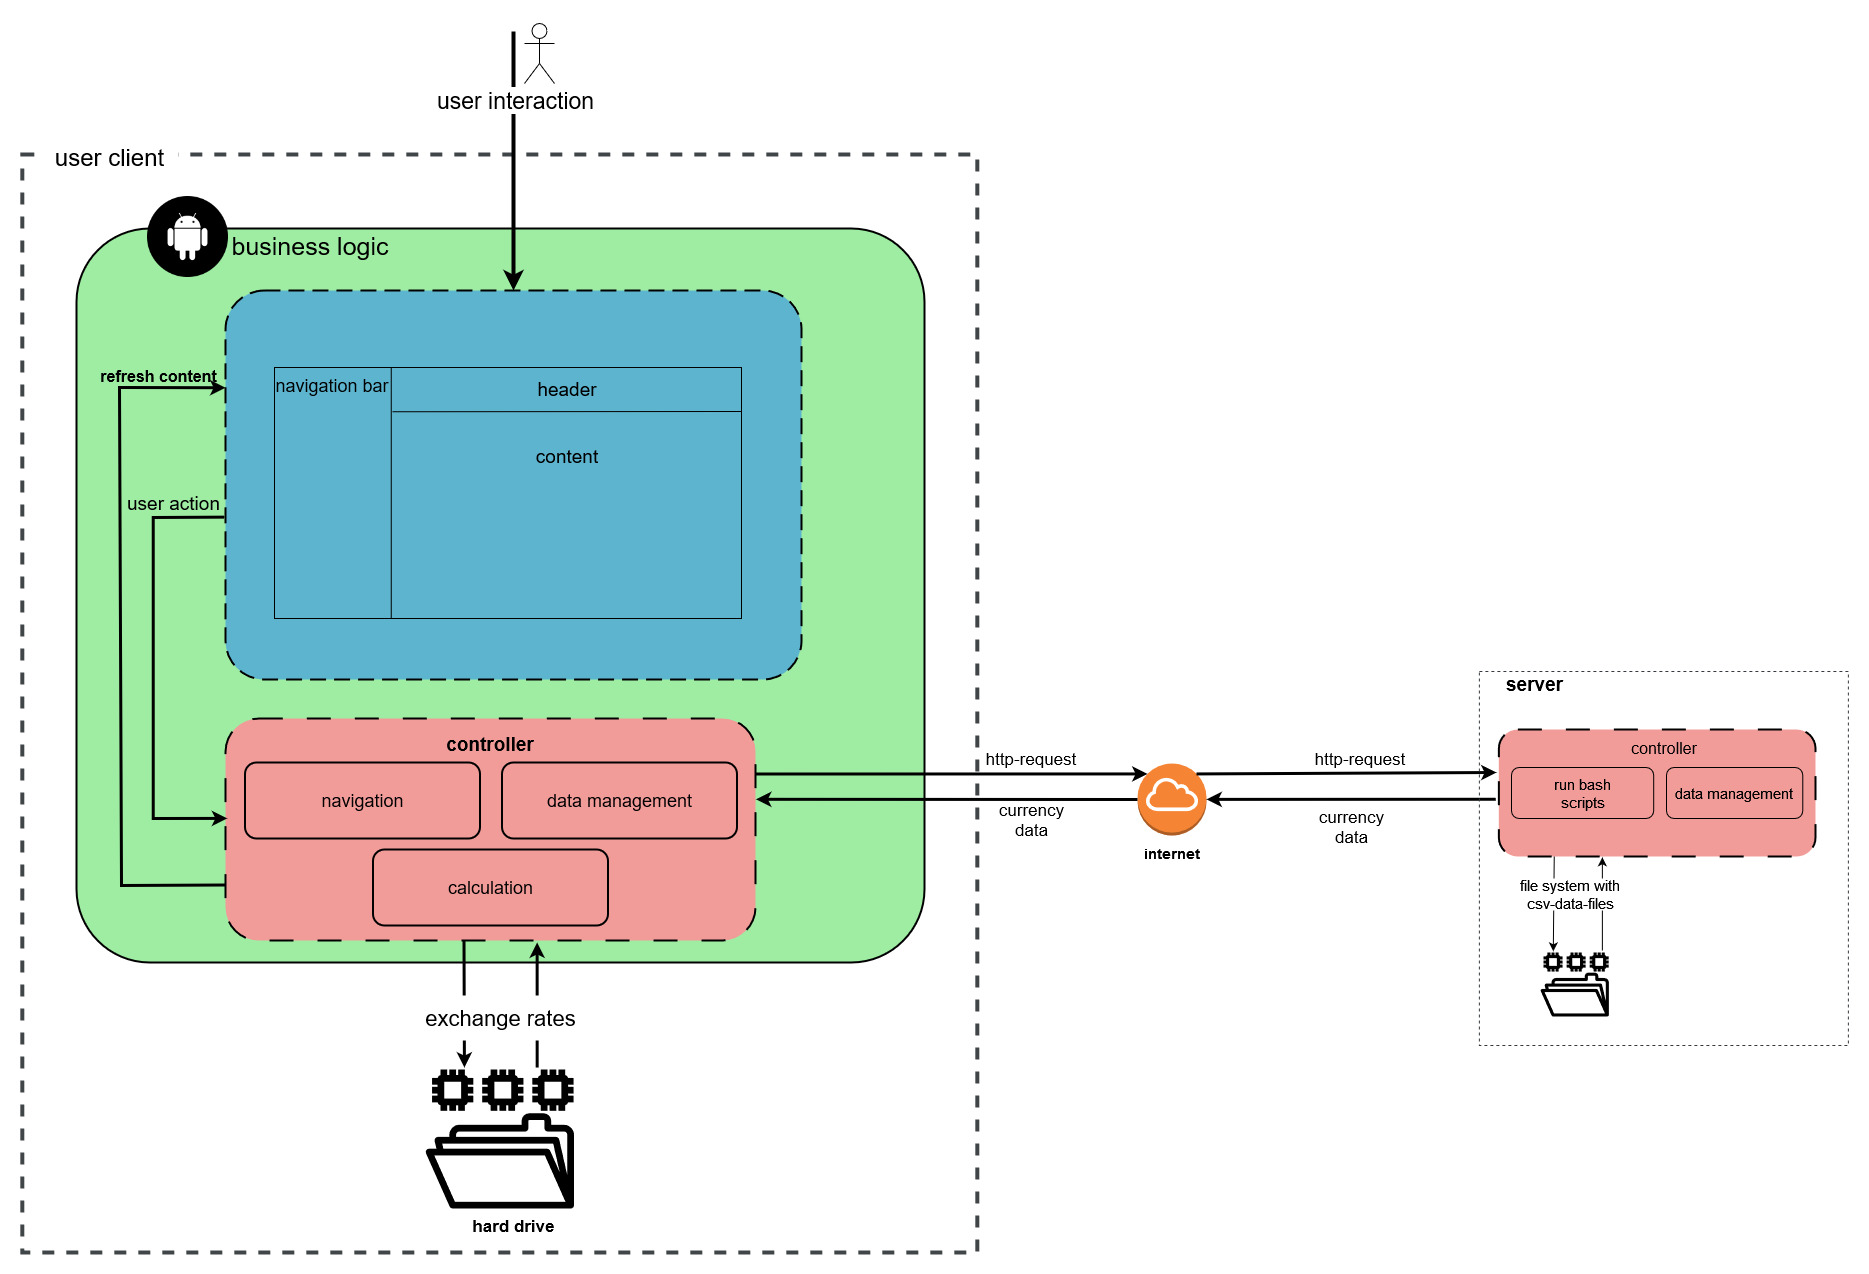
\includegraphics[width=1\linewidth, frame]{Software-Architektur_SWEII}
	\caption[Softwarearchitektur]{Softwarearchitektur}
	\label{fig:software-architektursweii}
\end{figure}
\noindent
Abbildung \ref{fig:software-architektursweii} zeigt wie die Softwarearchitektur strukturiert ist. Auf der linken Seite des Bildes ist der User-Client abgebildet und auf der Rechten der Server. Da die Software somit zwei Komponenten aufweist, handelt es sich um eine Zwei-Tier-Architektur. \\
Im User-Client ist zusehen, dass der User mit der in blau gekennzeichneten View interagiert. Die View ist das was die Nutzenden sehen können. Es besteht aus einem Header, einer Navigationsleiste, und dem Inhalt. Über die Interaktion mit dem View können Nutzende verschiedene Controller erreichen, die im roten Bereich zu sehen sind. In dem User-Client existieren drei unterschiedliche ein mal der Navigator, der Data-Manager und der Calculator. Der Data-Manager ist dafür zuständig die Daten in einem Ordner zu speichern und sie den Anderen Controllern bereit zustellen. Er stellt auch Anfragen per HTTP-Request an den Server. Der Calculator berechnet die Wechselkurse und der Navigator sortiert Daten und stellt sie dem View bereit, der sie dann anzeigt. \\\\ Der Server weißt auch Controller auf. Er hat Bash-Skripte, die den Webscraper steuern. Der Data-Manager ist hier auch wieder für die Aufarbeitung der Daten zuständig. \\\\ Der Webscraper wurde nicht in dem User-Client integriert, da somit zu viele Anfragen auf die Webseite verhindert werden können. Sollten zu viele Anfragen an die Webseite geschickt werden, kann es zu einer Überlastung dieser kommen und sie stürzt ab. Da sie nicht Eigentum des Projektteams ist, muss dies verhindert werden, weshalb ein eigener Server zur Verfügung gestellt wird. Bei dem ist es nämlich in Ordnung, falls er überlastet sein sollte, da der Server dem Projektteam durch Benjamin Liebenberg zur Verfügung gestellt wird.

\subsection{Sequenzdiagramm}
Das Squenzdiagramm beschreibt die Kommunikation der unterschiedlichen Instanzen innerhalb der Software. \newline

\begin{figure}[h]
	\centering
	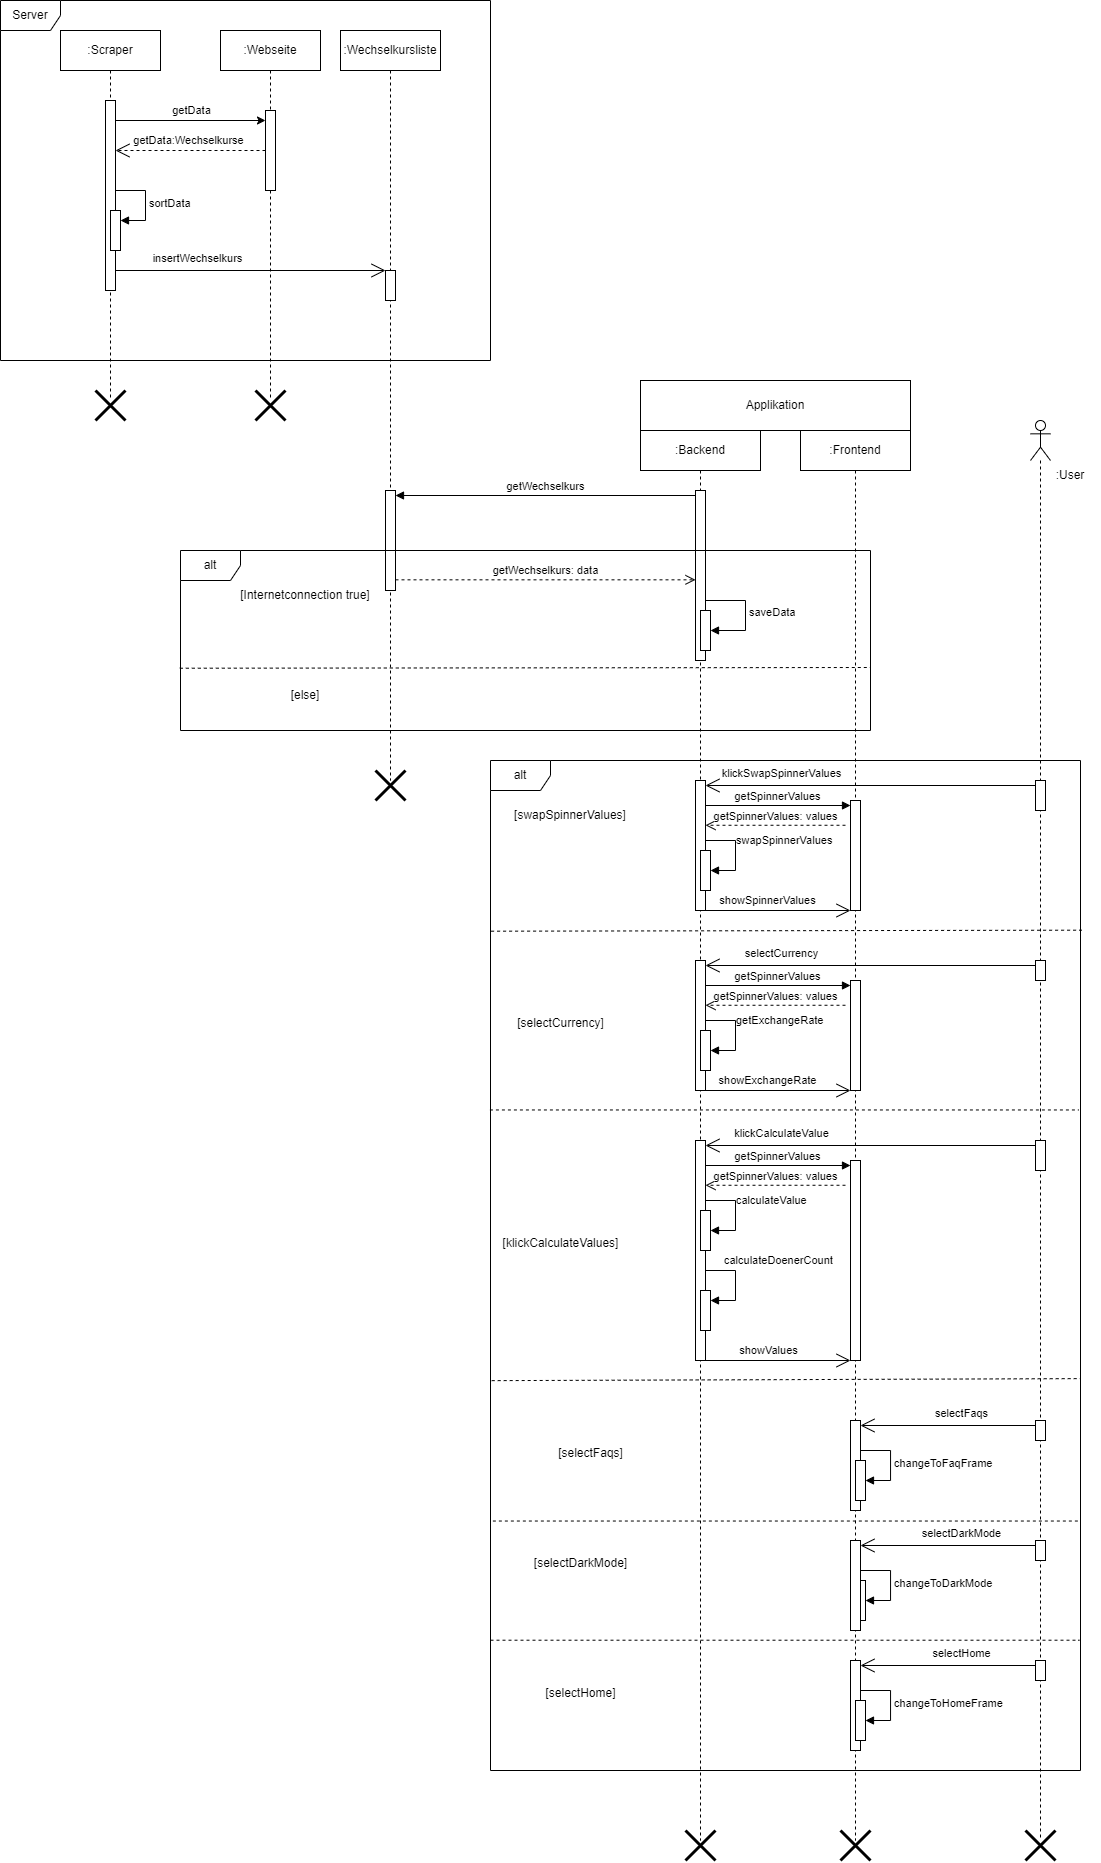
\includegraphics[width=1\linewidth, frame]{Sequenzdiagramm.drawio}
	\caption[Sequenzdiagramm]{Sequenzdiagramm}
	\label{fig:sequenzdiagramm}
\end{figure}
\noindent
Abbildung \ref{fig:sequenzdiagramm} zeigt auf, wie das Sequenzdiagramm gestaltet worden ist. Oben links ist der Serverbereich. Der Webscraper holt sich die Daten von einer Webseite und strukturiert sie. Danach werden diese dann in einer CSV-Datei gespeichert. Etwas weiter unten ist die Applikation, die wiederum in ein Front und in ein Backend geteilt ist. \\\\ Das Backend schickt eine Anfrage an den Server um die SCV-Datei zu erhalten. Sollte es eine Internetverbindung geben, erhält es diese und speichert sie ab, wenn nicht werden die Altdaten der Applikation weiter verwendet. \\\\ Unter der Abfrage ist ein alt Feld zusehen, welches alternativ Möglichkeiten der User-Applikation-Interaktion bereitstellt. Die ersten drei Optionen haben eine ähnliche Struktur. Die nutzende Person schickt eine Anfrage an das Backend. Dieses holt sich dann Daten aus dem Frontend. Danach kommen dann die Unterschiede bei den ersten drei Möglichkeiten zum Vorschein. Wenn die Werte getauscht werden sollen, tauscht das Backend die Werte. Wird eine neue Währung gewählt, sucht es den neuen Wechselkurs heraus. Soll eine Umrechnung stattfinden wird zuerst der Betrag in der Währung und dann die Anzahl der Döner berechnet. Danach sind die Möglichkeiten wieder identisch, denn das Backend schickt daraufhin eine Nachricht an das Frontend, welches die neuen Daten dann anzeigt. \\\\ Die letzten drei Möglichkeiten weisen untereinander auch wieder Ähnlichkeiten auf. Die Nutzenden schicken eine Anfrage an das Frontend, welches sich dann verändert. Die drei Möglichkeiten sind die Auswahl des Home-Seite, der FAQ-Seite und der Wechsel von und zum Dark-Mode.

\section{Implementierung}
Die Implementierung ist in drei Abschnitte geteilt. Diese Segmente sind die Implementation der App, des Servers und die Verbindung der beiden Komponenten.

\subsection{Implementierung der App}
Zur Implementierung der App wurde Android-Studio verwendet, welches eine Entwicklungsumgebung zur Entwicklung von Android-Apps ist. Innerhalb der Umgebung kann zwischen zwei Programmiersprachen gewählt werden. Diese sind Java und Kotlin. Zur Entwicklung der App wurde Java gewählt, da das Projektteam bereits Erfahrungen mit Java  durch das Modul Objekt orientierte Programmierung im zweiten Semester sammeln konnte. \\\\ Innerhalb der Java-Dateien wurde die Business-Logik implementiert. Die Darstellung der App kann auch mithilfe von Android-Studio übernommen werden. Dazu wurde in sogenannten XML-Dateien die Darstellung erstellt.

\subsection{Implementierung des Servers}
Nach der Einstellung des Servers wurde ein C\#-Skript entwickelt, welches für den Webscraper und die Datenstrukturierung zuständig ist. Es greift  auf eine Webseite zu und lädt die dortige HTML-Datei herunter. Danach liest es aus der Datei alle relevanten Daten und strukturiert diese. Nach der Strukturierung werden sie dann in einer CSV-Datei auf dem Server gespeichert. \\\\ Damit das C\#-Skript nicht jeden Tag manuell ausgeführt werden muss, wurde zusätzlich ein Bash-Skript entwickelt. Dieses Skript ist dazu zuständig jeden Tag um 6 Uhr das C\#-Skript auszuführen. \\\\ Nach der Erstellung der Skripte wurde zusätzlich eingestellt, dass die entstandene CSV-Datei über die IP-Adresse des Servers und einem Port zugänglich ist.

\subsection{Verbindung zum Server}
In der App wurde implementiert, dass sie eine Anfrage an den Port des Servers schickt, unter dem die CSV-Datei erreichbar ist. Sollte eine Internetverbindung vorliegen, wird die sie heruntergeladen und gespeichert.

\section{Integration}

\section{Tests}

\section{Wartung}

\section{Rollout}

\section{Ergebnis}

\section{Abschluss}



\end{document}
